% Chapter 1

\chapter{Development Methodology} % Main chapter title

\label{Chapter2} % For referencing the chapter elsewhere, use \ref{Chapter1} 

\lhead{Chapter 2. \emph{Development Methodology}} % This is for the header on each page - perhaps a shortened title


This project differed from traditional software development projects in that children participate in the process of designing the interactions and applications that were created. In pursuing and developing this research project, I worked with KidsTeam which is an intergenerational design team  directed by Dr. Jerry Alan Fails where children and adult researchers work together as design partners in a collaborative and elaborative process. The children affiliated with this particular group participated in the application's design process. Because of this collaboration, the project's development process was different from the traditional projects in the way the phases were performed and required a very flexible model of development. 

\section{KidsTeam}
The KidsTeam is a group of eight children ages 6 to 11, male and female, directed by Dr. Jerry Alan Fails at Montclair State University. The group meets twice a week for one and a half hour (4-5:30pm) sessions over the course of a semester. During that time, the KidsTeam worked on various projects which were facilitated by Dr. Fails along with several undergraduate and graduate students. The objective is to leverage the children's natural capacity for divergent thinking in a collaborative environment to develop an application for the LeapMotion. In order to achieve an optimal outcome, the professor and students created a community of respect and rapport. The purpose is to create a safe space where the children felt free to explore and share their ideas. Therefore, it is imperative that the atmosphere remain relaxed. The atmosphere is purposefully not like school, and measures are taken to equalize the power structures that are generally inherent in adult-child relationships and instead build a relationship of mutual respect and trust, thus facilitating a fluid working relationship.

%This is enforced by rules that framed particular behaviors such as encouraging the children to speak when they have a thought, idea, or question rather than raising one's hand. The only strict requirement of the children during the sessions is that they must respect everyone, including the adults, in KidsTeam. 

KidsTeam creates a dialog when designing and developing an application between the developers and the users by building off each others ideas. This intergenerational design team collaborates by exchanging ideas and giving opportunities to enhance every aspect of the application. 

\section{Collaboration Techniques}
Several techniques were implemented in order to aid the development process. These techniques were chosen for their means to foster a community of cooperative inquiry where the children felt encouraged to contribute design ideas freely. \cite{journalsjcalScottMI03}\cite{Colella98}

%These techniques are designed to encourage children to freely contribute while divergently thinking to contribute design ideas. \footnote{Out of Our Minds}

\subsection{Sticky Notes}\label{sec:stickynotes}

\begin{figure}
\centering
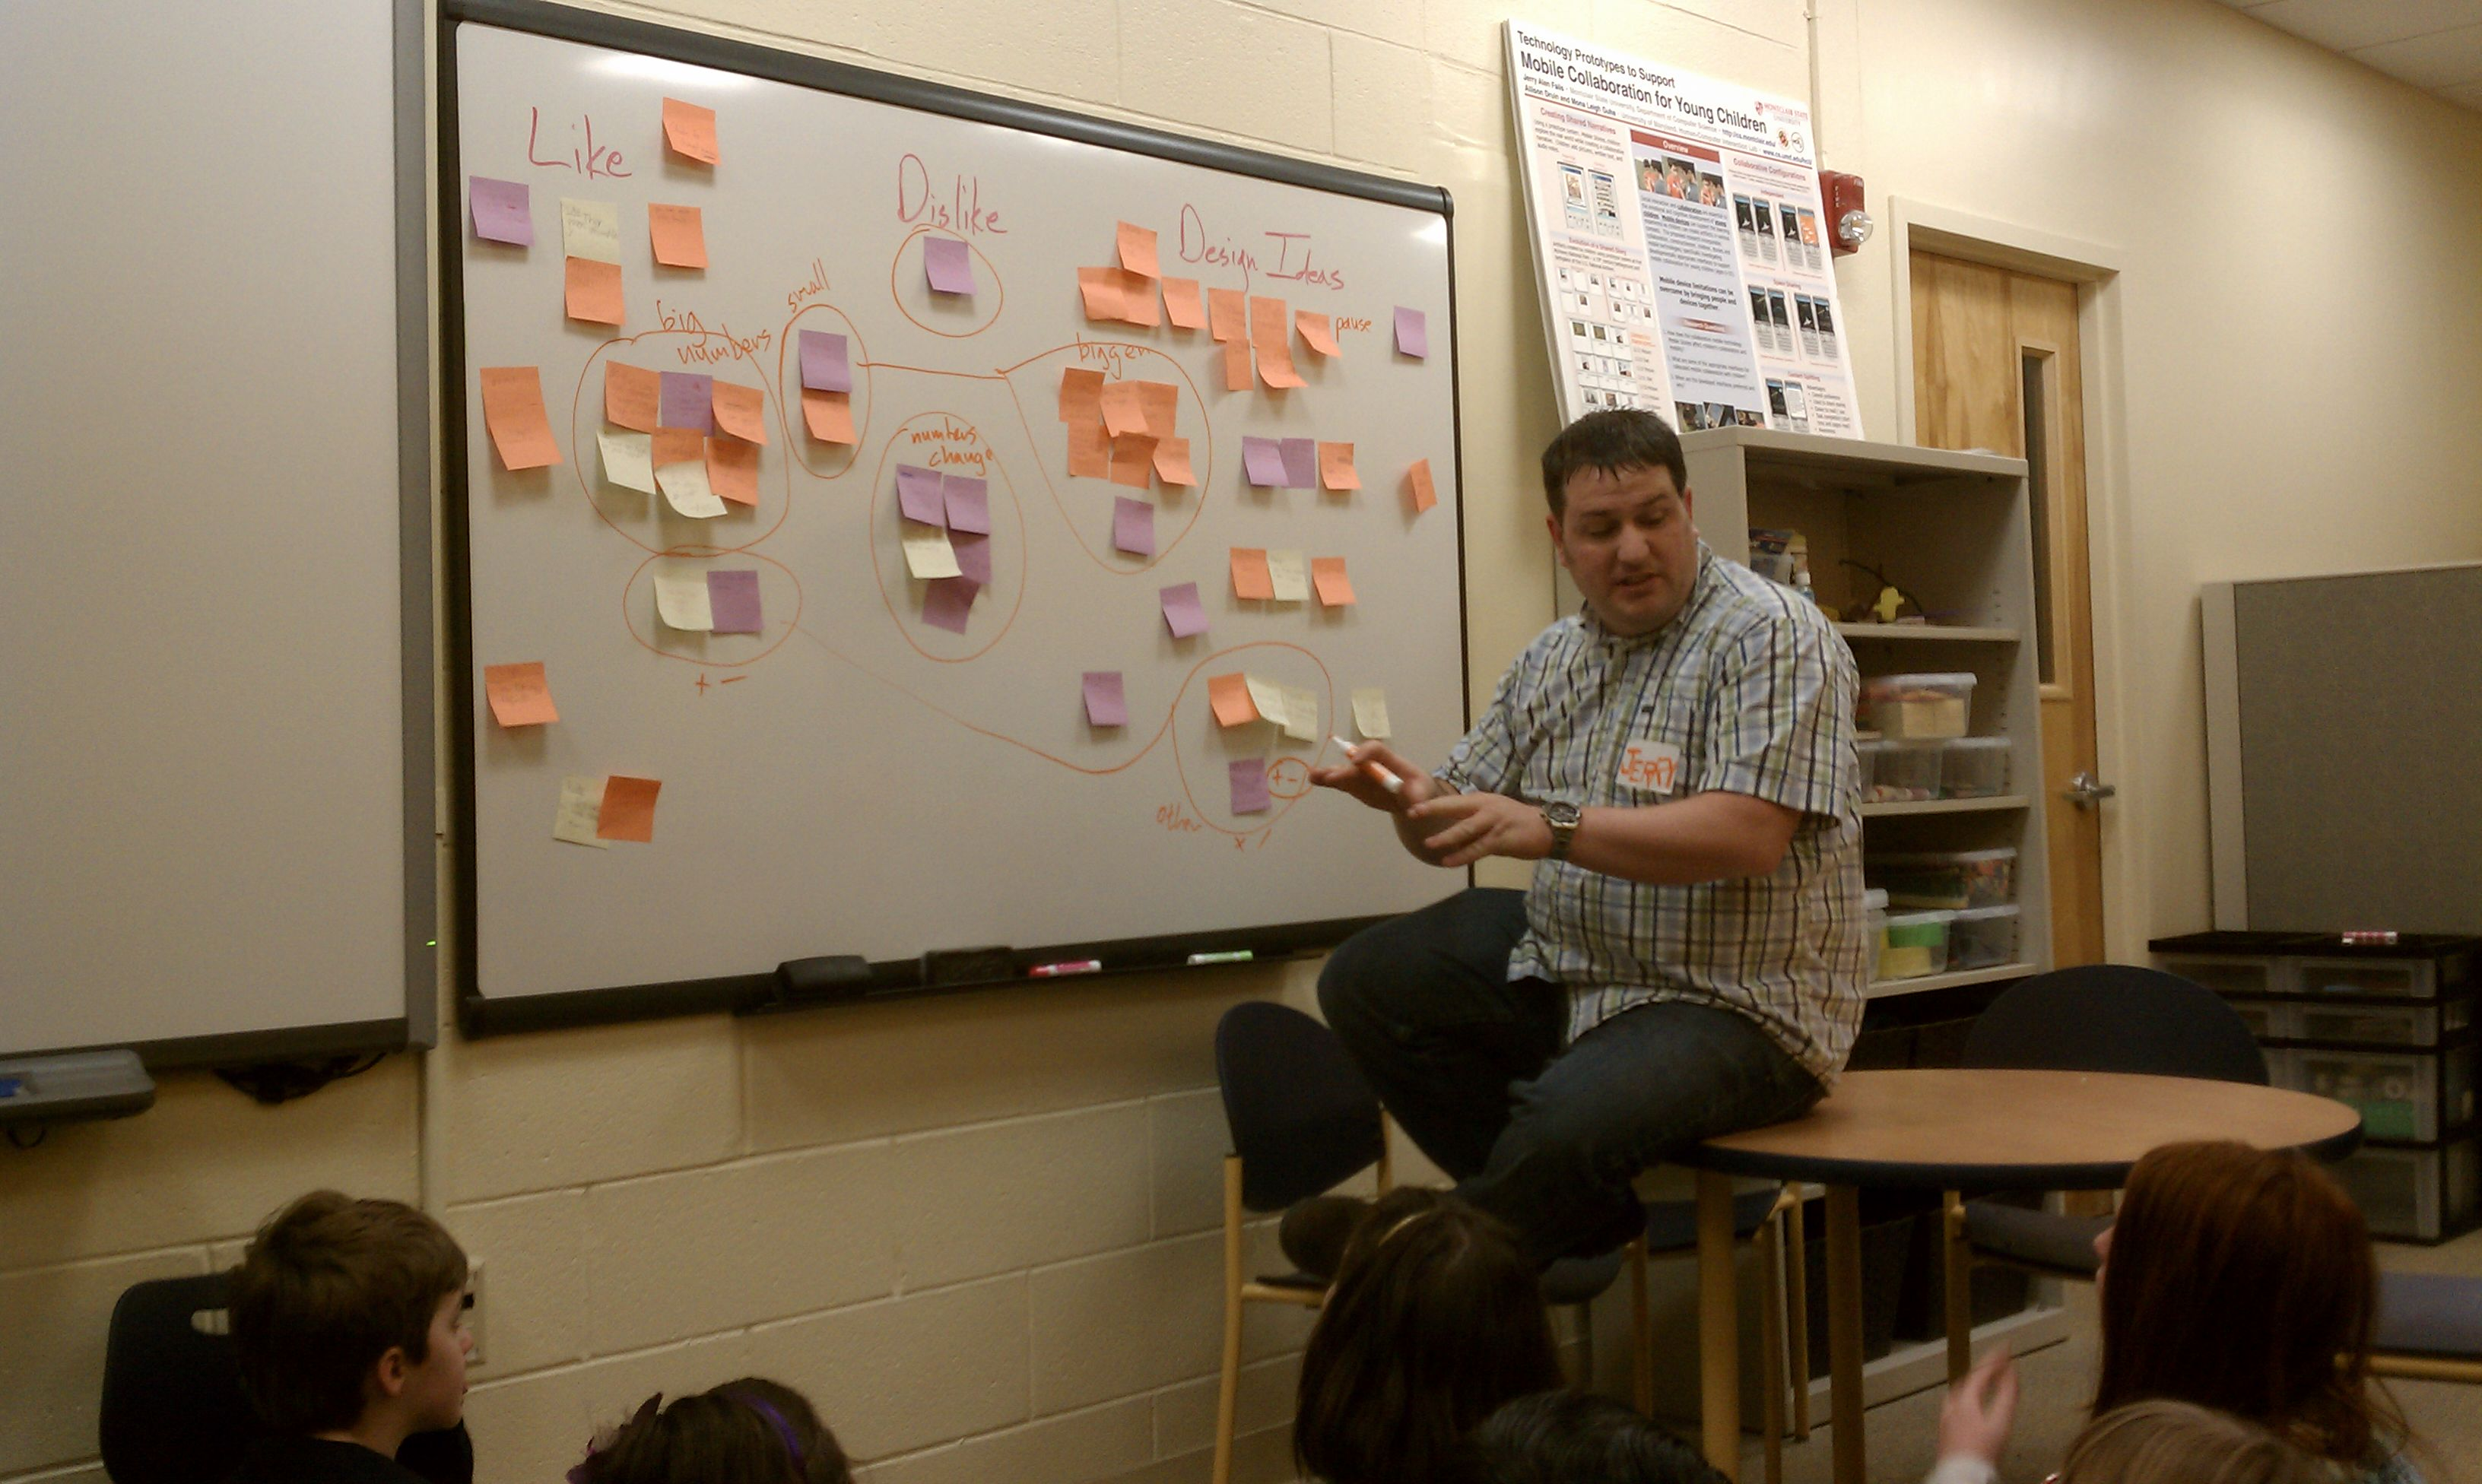
\includegraphics[height=1in, width=1.5in]{IMAG0270}
%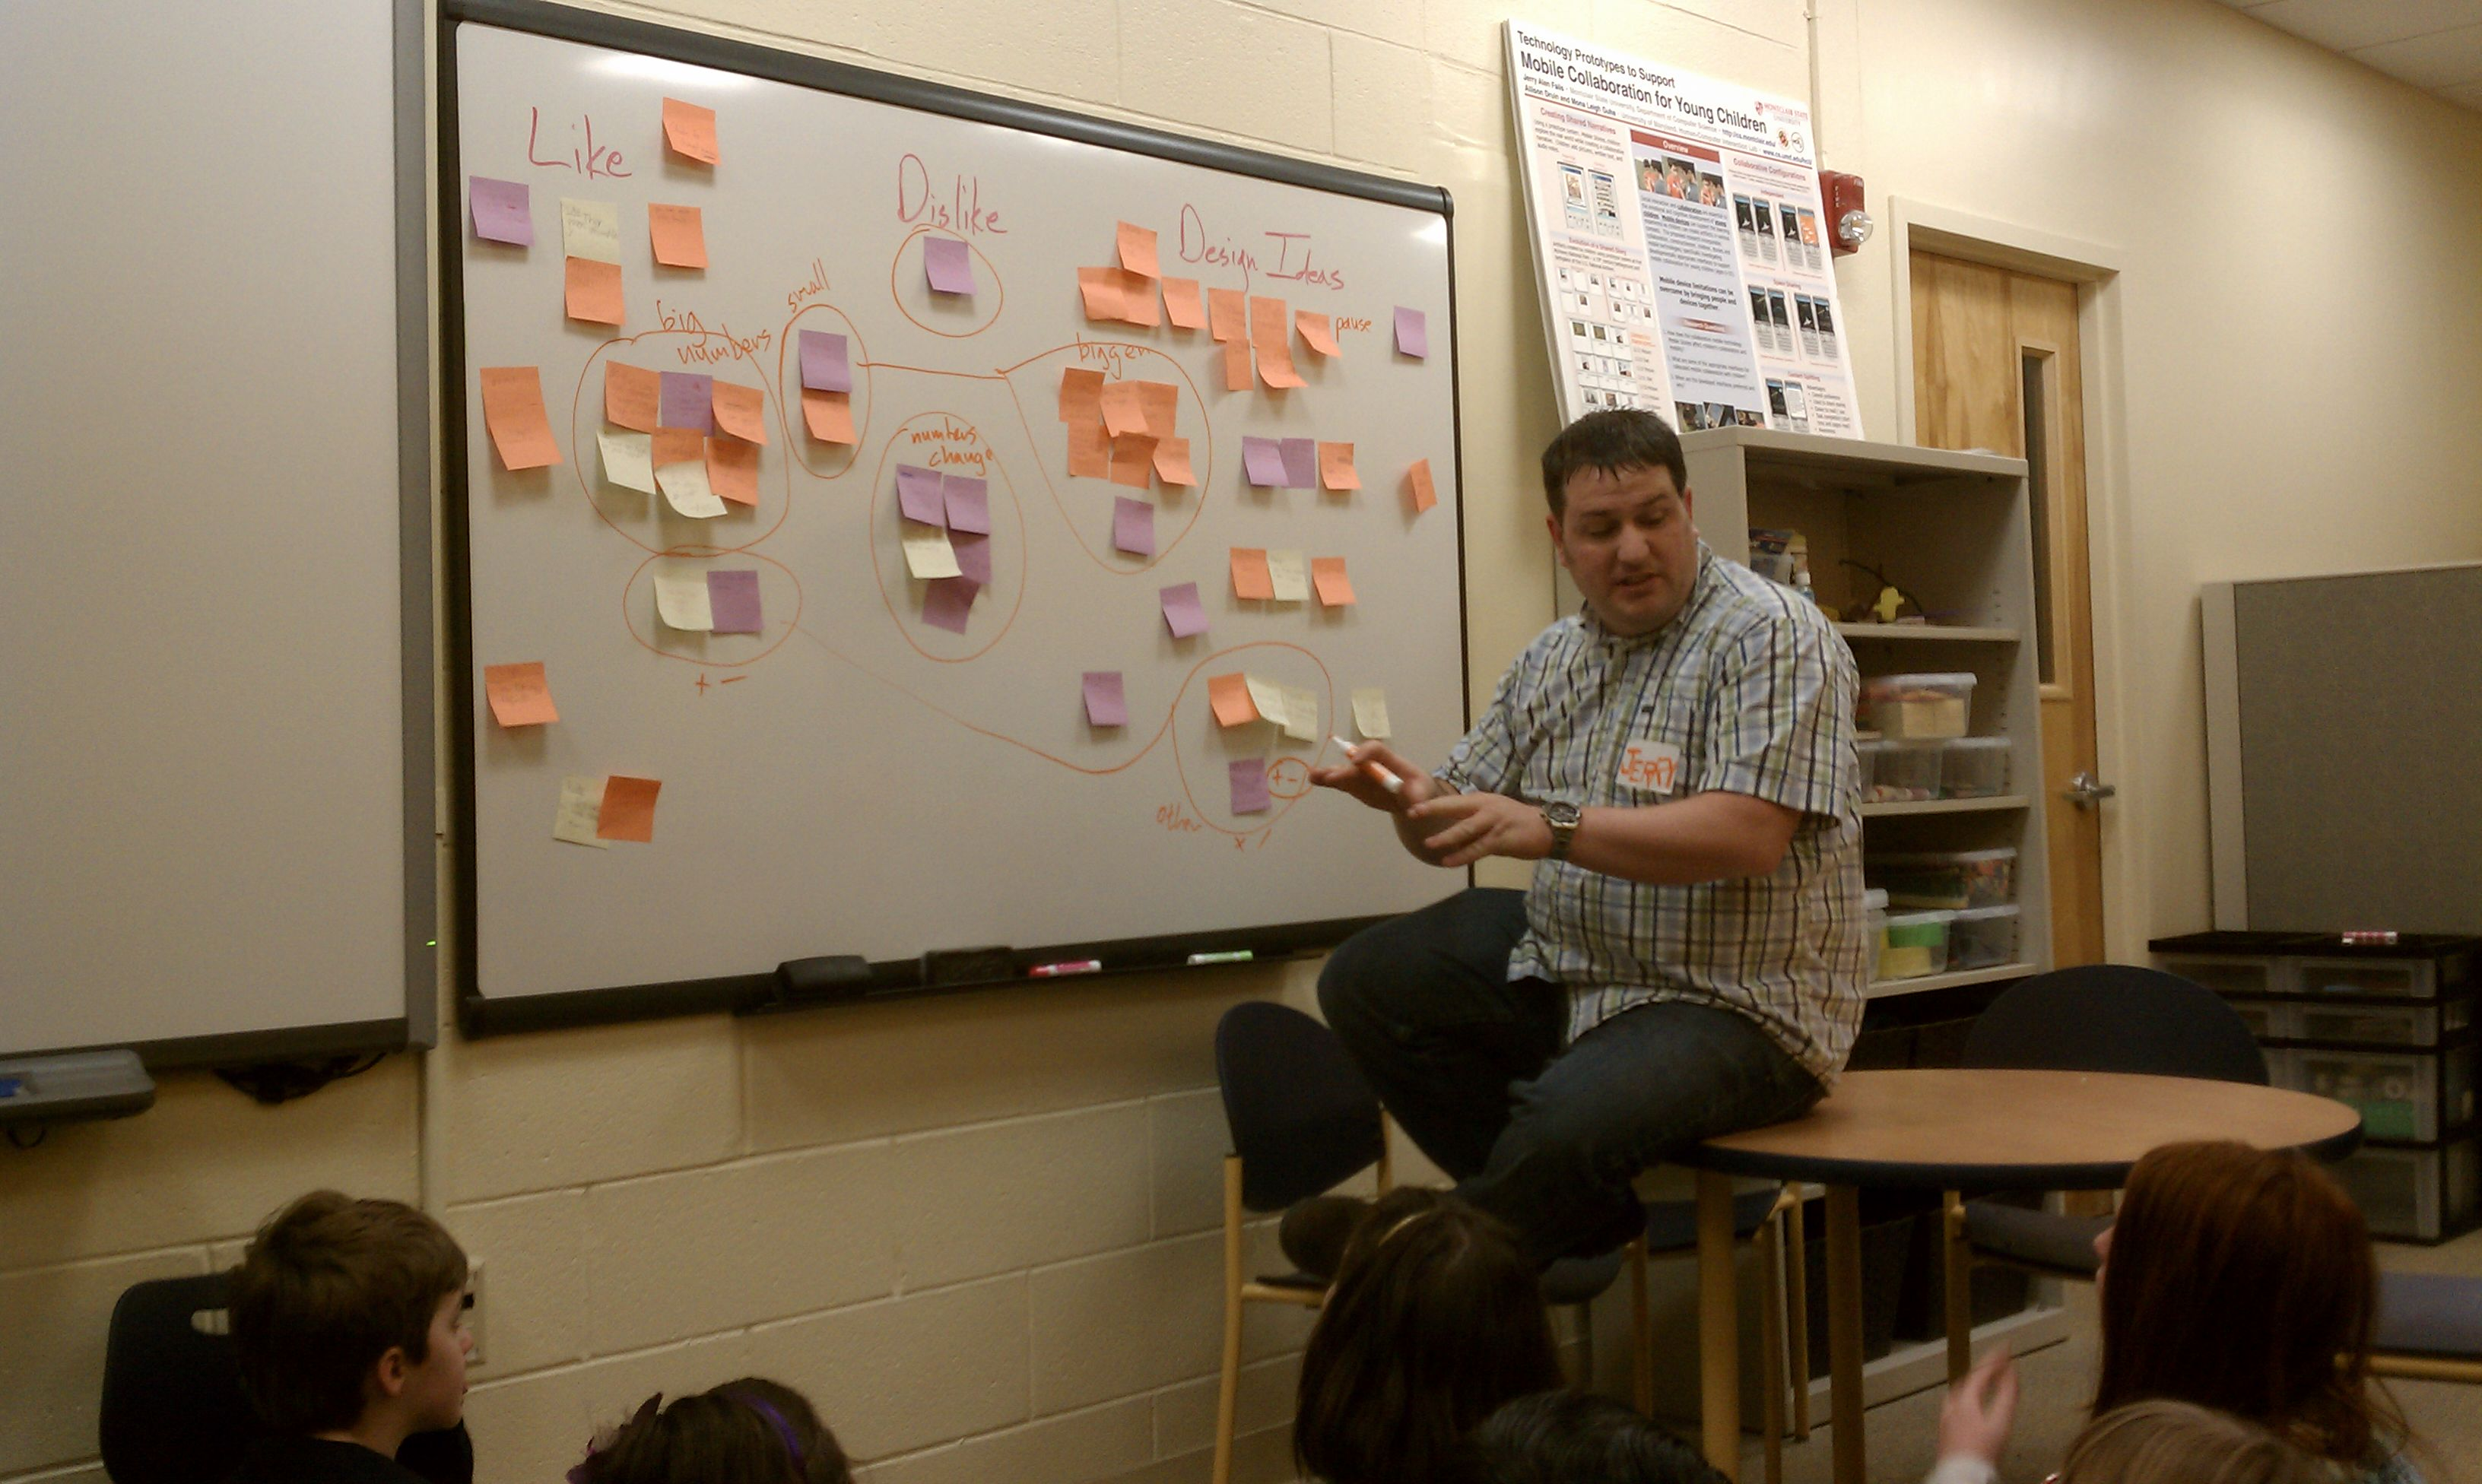
\epsfig{file=IMAG0270, height=1in, width=1.5in}
\caption{Reviewing the sticky notes using a spatial graph on a white board for easy comparison and analysis. }
\label{fig:stickynotesreview}
\end{figure}

Each child was given a pad of Post-It notes\footnote{Small square of paper with adhesive on reverse side.}.During activities which required comment, as the children played with the cubes, the children would write comments on the PostIt notes\footnote{One comment per sticky note.}. These comments were categorized into like, dislike, or design idea and then stuck to the white board. A facilitator would then organize the notes based on the category and the comment content to resemble a spatial graph where similar comments are grouped closer together, while outlying comments are spread farther apart. Comments relating to a specific function or component are arranged into the same row while the category of the comment will determine the column. At the end of the session the observer debriefs with the children about the session by reviewing the comments arranged on the white board and having the children comment about the session overall. This time allows for the observer and the children to summarize the session, gives the children extra time to comment and provide more specific feedback, and permits the observer to further clarify a child's reasoning for making certain comments. The result is a frequency analysis as seen in Figure~\ref{fig:stickynotesreview} which feedback can be turned into specifications for the next design cycle.  \cite{Druin:1999:CID:302979.303166}\cite{Druin02therole} 

\subsection{Bags of Stuff} \label{sec:bagsofstuff}
Each child is given a Bag of Stuff that contains a variety of arts and crafts supplies such as Popsicle sticks, felt, construction paper, markers, etc. The children are then given a design concept by the observer and asked to use these materials to construct that concept. As the children build, they must explain in their own words how their concept works while the observer takes notes. \cite{Druin:1999:CID:302979.303166}\cite{Druin02therole}

\subsection{Storyboarding}\label{sec:storyboarding}

The children are split into groups. The groups were chosen at random and did not remain intact from session to session. Each group then receives one large piece of construction paper. They will use the paper, sticky notes, and markers to draw their particular game concept sequence of events. Any actions or changes in a scene must be drawn in the order that they occur. The children must use arrows to delineate the progression of events. In order to make sure their ideas are conveyed clearly, the children are asked to be as descriptive as possible while facilitators take notes as the children work. \cite{Druin:1999:CID:302979.303166}\cite{Druin02therole}

\section{Development Model}
Working with KidsTeam required a lot of flexibility in the development process and is why Rapid Application Development (RAD) model\footnote{Iterative or incremental development process resembling an evolutionary pattern.} for software development was chosen as the best fit model for this project. The RAD model uses rapid prototyping\footnote{Rapid Prototyping will produce a quick mockup for testing in each cycle.} and continuous iterative cycles which allowed for testing with KidsTeam on a weekly basis. Each session with the KidsTeam generated new requirements and fixes to be implemented within tight time constraints prior to the next session.

The model centered around five phases: Specification, Design, Code, Test and Review as seen in Figure~\ref{fig:agiledesignprocess} constituting a full cycle. Changes in the specification were then implemented and reflected in the application prototypes ready for the next session. Each session with KidsTeam marked the end of current cycle and start of the next in the development process. \cite{0136061699}\cite{Ruparelia:2010:SDL:1764810.1764814}

The children were most heavily involved in the specifications, design, test and review phases in each of the nine sessions. Some parts of the design and testing were done independently of the children but mostly cosisted of elaborating on either their designs and ideas or were performed to ensure the application was stable enough for testing with the children.  

%Agile foot note and reference if it can be included  K. Reed, E. Damiani, G. Gianini, and A. Colombo.
\begin{figure}
\centering
%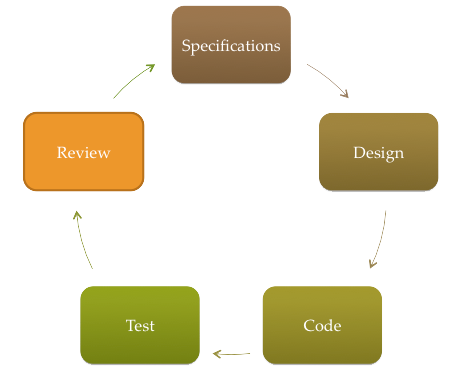
\epsfig{file=agiledevelopment2, height=0.95\columnwidth, width=\columnwidth}
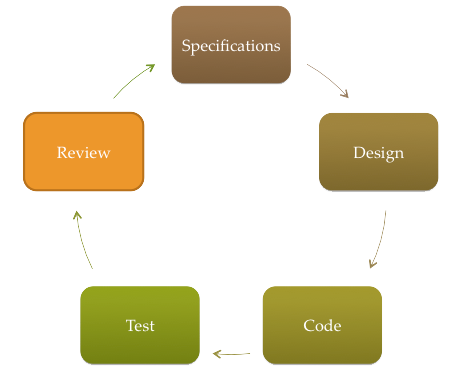
\includegraphics[height=0.5\textwidth, width=0.5\textwidth]{agiledevelopment2}
\caption{Rapid Application Development cycle \cite{Ruparelia:2010:SDL:1764810.1764814} }
\label{fig:agiledesignprocess}
\end{figure}


\subsection{Specification}\label{sec:specificationphase}
The specification is the set of requirements for the application's functional components and use cases. This includes what the application must be able to do and defines the parameters the application must operate within. 

\subsection{Design}\label{sec:designphase}
 The design takes the specification and frames a way to implement them in the next phase of coding. This includes how the user interface will be laid out, components will function and the architecture of how each component will interface to become a working application that will fulfill the specification requirements.  

\subsection{Code}\label{sec:codephase}
Coding is the process of taking the design and implementing it into functional units of code that run the application. The code will contain models of objects, actions, responders, delegates and flow control of application.

\subsection{Test}\label{sec:testphase}

Includes writing test cases for the functional components and debugging issues within the code such that the application meets the requirements in the specification. This process was done by the developer to ensure the application is stable enough for the children to perform fullstack testing of the application.

\subsection{Review}\label{sec:reviewphase}

After testing was performed by KidsTeam, the children provided direct feedback via the sticky notes collaboration technique. A frequency analysis of the sticky notes determined the next set of requirements for the specifications in the upcoming cycle. 

\section{Progress Updates}
%Done via the wiki and Youtube updates
Throughout the course of the project updates were posted on a wiki and on youtube. Each wiki update summarized the session with the children including goals, observations and new requirements taken from the session along with pictures of the session. Videos posted on youtube mostly described major changes within the application itself and intermediate project updates.

Source code was kept in a public github repository\footnote{Due to the number of prototypes, the repositories were later consolidated into one repository.} along with the project documentation. Any additional project documents were kept here. 

